Version 1 largely adheres to the design specification.

\begin{figure}
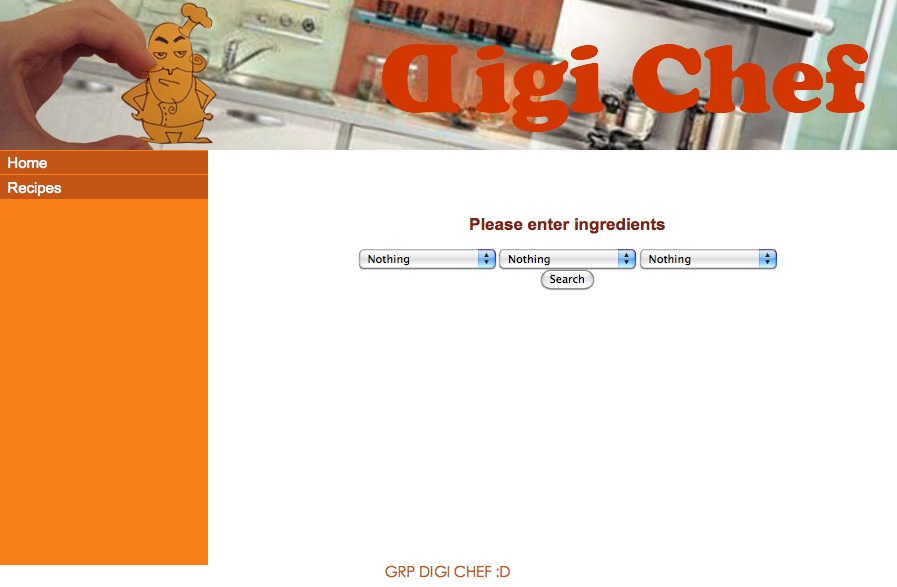
\includegraphics[width=0.9\textwidth]{result_1}
\caption{Homepage}
\label{fig:result_1}
\end{figure}


As mentioned, white and orange are the colours of choice, along with an appealing logo. The design is simple and effective in meeting the needs of version 1.(Fig~\ref{fig:result_1}) shows the drop down menus for ingredient selection with the search option.

(Fig~\ref{fig:result_2}) shows the result of ingredient selection by the user. The recipe list was generated based on the ingredients selected by the user.

\begin{figure}
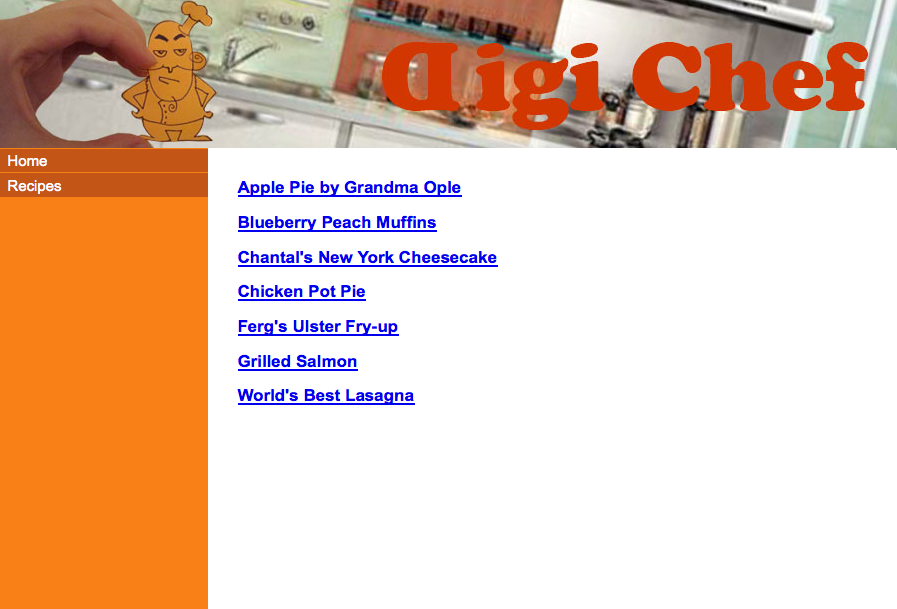
\includegraphics[width=0.9\textwidth]{result_2}
\caption{Search results}
\label{fig:result_2}
\end{figure}

(Fig~\ref{fig:result_3}) shows the result of clicking on a recipe. Notice the Recipes button on the far left hand side of the web page. Clicking that generates the list of all recipes in the database.

\begin{figure}
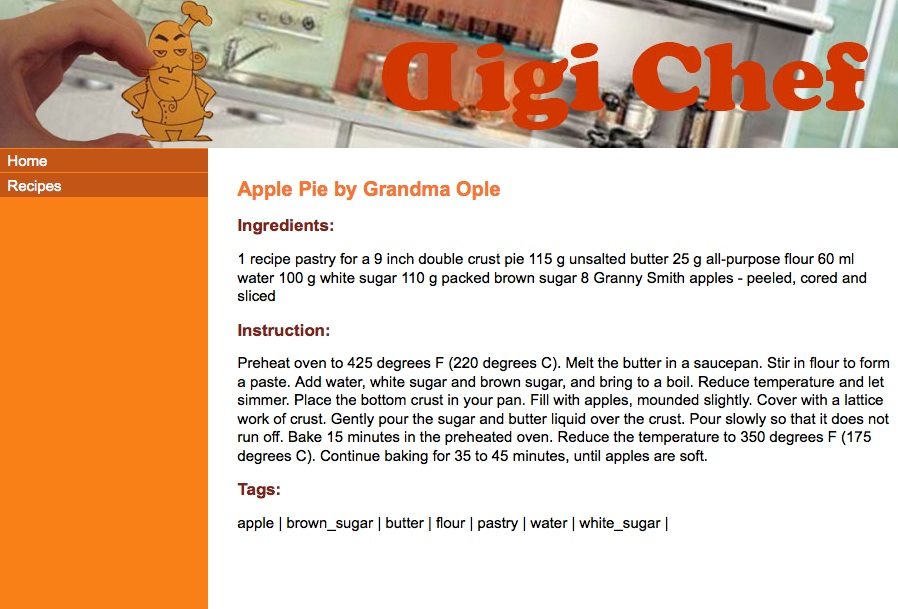
\includegraphics[width=0.9\textwidth]{result_3}
\caption{Recipe page}
\label{fig:result_3}
\end{figure}

The group thoroughly scoured the website of bugs by doing exhaustive testing of all the possible ingredients and checking if the returned list matches the input ingredients. Exhaustive testing was possible for version 1 due to the small database and only three ingredient boxes. However, as our system gets more complicated, this form of testing will be unwieldy. A better method of testing will be required then.


\subsection{Version 2 Implementation}

The main addition to Version 2 was the much more advanced collaborative filtering functionality.

\subsubsection{Collaborative filtering implementation}

The implementations of collaborative filtering methods in the module \texttt{django-recommender} were not as suitable for our needs as they first appeared, and had to be modified.

Some of these modifications were simple, for example there was no easy way to search for a recipe based on a set of tags, which we needed to implement search. A new method was adapted from an existing method which found items similar to a given item. The original method used the tags of the given object to do the similarity comparison, so the new method skipped the stage of extracting the tags from the given object and had the tag list be passed in as an argument in place of the object.

Others were more difficult. The method designed to recommend recipes to users was designed to work on tagged users. The idea here was that users would tag themselves with things they like. For example in a film rating system, action fans would tag themselves with `action', the same `action' tag applied to action movies. In this context that made little sense, as people are rarely `fans' of individual ingredients, and no-one is going to want to tag themselves `onion'. So I wrote my own rating prediction function based on the equations in the collaborative filtering research section of the report, from scratch.

The method I used was the final user-based nearest neighbour method in the research:

\begin{equation}\label{eq:avgadjust}
pred(u,i) = \overline {r}_u + \frac{\sum_{n\subset neighbours(u)} userSim(u,n)~\cdot~(r_{ni}-\overline {r}_n)}{\sum_{n\subset 
neighbours(u)}userSim(u,n)}
\end{equation}

A direct translation of this function into code was implemented. This proved to be extremely inefficient, taking approximately 1.5 to 2.0 seconds to rate each recipe, suggesting a total recommendation time for the database of 24 to 31 minutes. This was obviously unacceptable, so optimisations were sought.

A lot of things were being unnecessarily recalculated each time. Some of these things, like average vote for a user, or a 1-dimensional array of all votes for a user, could be calculated once per vote and stored in the database, so these calculations were moved to the voting part of the operation. This introduced a small delay in voting, which is far less of a problem than it would be here, because voting is done with \textsc{Ajax}, so the user isn't interrupted, and voting is very fast anyway. These re-factorings made the method run in one tenth the original time.

Some things, like the sum of similarity ratings to neighbours, had to be calculated each time recommendations were sought, but not for each recipe, so these were moved to be pre-calculated before the loop over recipes. Moving out the similarity sum calculations doubled the running speed again, and pre-calculating individual user similarities caused further drastic speed increases. The final implementation operated 171 times faster than the original.


